\documentclass{beamer}
\usepackage{graphicx}
\usepackage{amsmath, esint}

\usepackage{tikz}
\usetikzlibrary{arrows,shapes}

\usepackage{algorithm}
\usepackage{algorithmic}

\usepackage{xcolor} 
\definecolor{LightGray}{gray}{0.975}

%\usetheme{Warsaw}
\usefonttheme{serif} 

\title[Chapter 2]{Database System Concepts, $7^{th}$ Edition \\ Chapter 2: Introduction to Relational Model}
\author{Silberschatz, Korth and Sudarshan}
\date{\today}

\setbeamertemplate{navigation symbols}{}%remove navigation symbols

\defbeamertemplate*{footline}{shadow theme}
{%
  \leavevmode%
  \hbox{\begin{beamercolorbox}[wd=.5\paperwidth,ht=2.5ex,dp=1.125ex,leftskip=.3cm plus1fil,rightskip=.3cm]{author in head/foot}%
    \usebeamerfont{author in head/foot} Database System Concepts \hfill \insertshorttitle
  \end{beamercolorbox}%
  \begin{beamercolorbox}[wd=.5\paperwidth,ht=2.5ex,dp=1.125ex,leftskip=.3cm,rightskip=.3cm plus1fil]{title in head/foot}%
    \usebeamerfont{title in head/foot} \hfill \insertframenumber\,/\,\inserttotalframenumber%
  \end{beamercolorbox}}%
  \vskip0pt%
}

\AtBeginSection[]
{
     \begin{frame}<beamer>
     \frametitle{Plan}
     \tableofcontents[currentsection]
     \end{frame}
}

\begin{document}

\frame{\titlepage}

\begin{frame}{Database System Concepts}
    \centering
    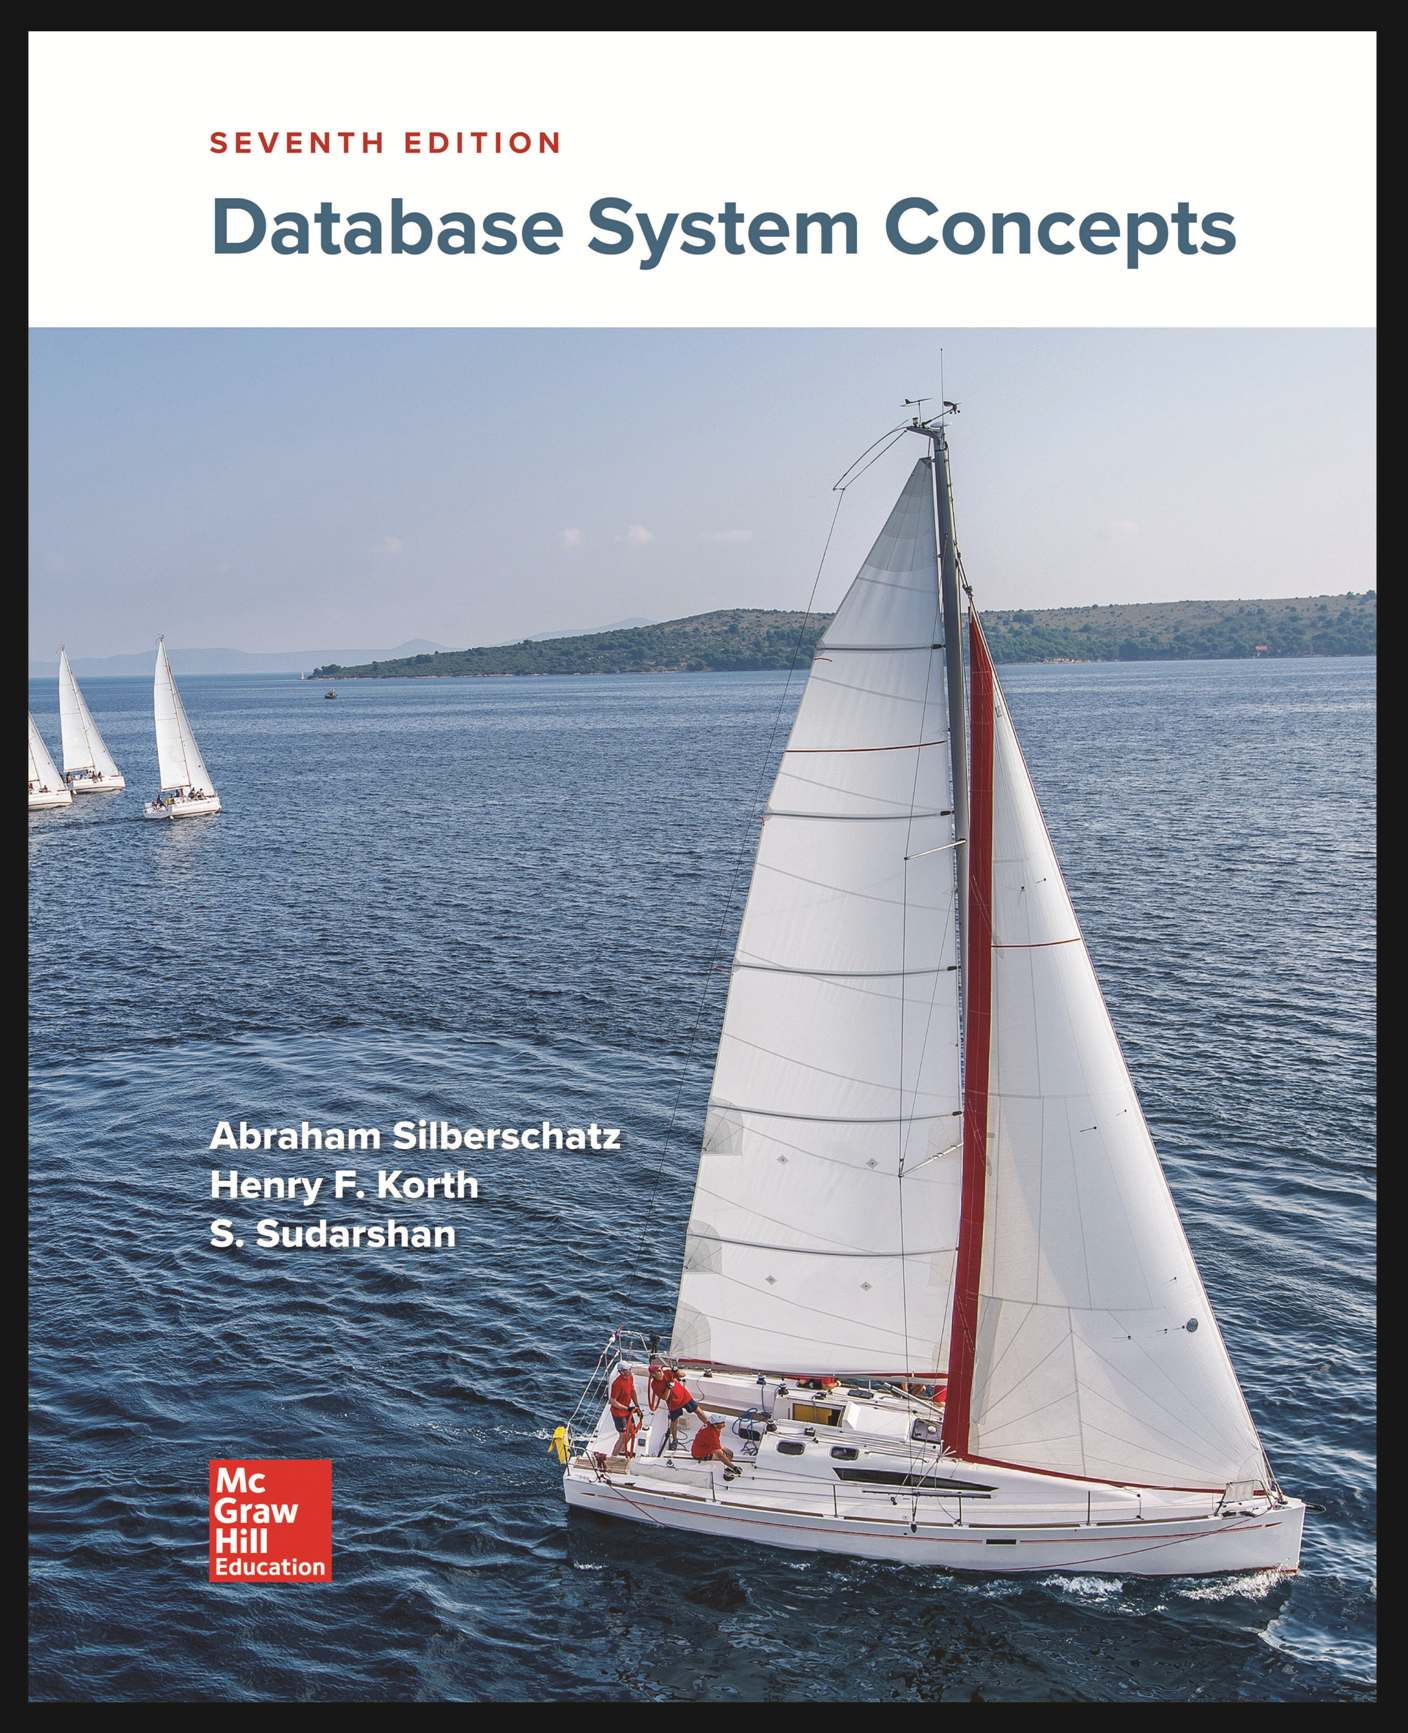
\includegraphics[width=0.5\textwidth]{figures/book_cover.jpg} \\
    \vspace{5mm}
    {
        \tiny
        Content has been extracted from \textit{Database System Concepts}, Seventh Edition, by Silberschatz, Korth and Sudarshan. Mc Graw Hill Education. 2019.\\
        Visit \url{https://db-book.com/}.\\
    }
\end{frame}

\begin{frame}{Example of a Instructor Relation}
    \centering
    \vspace{5mm}
    \includegraphics[width=0.65\textwidth, trim={7.25cm 16.75cm 6.5cm 4.75cm}, clip]{figures/Instructor_relation}
    \begin{tikzpicture}[remember picture,overlay]
        \node[] at (1, 6.75) {\tiny attributes (or columns)};
        \draw[red,thick,->] (0.10, 6.60) -- (-4.50, 5.55);
        \draw[red,thick,->] (0.10, 6.60) -- (-2.50, 5.55);
        \draw[red,thick,->] (0.10, 6.60) -- (-0.75, 5.55);
        \node[] at (1, 4.75) {\tiny tuples (or rows)};
        \draw[blue,thick,->] (0.05, 4.75) -- (-0.63, 4.77);
        \draw[blue,thick,->] (0.05, 4.75) -- (-0.63, 4.47);
        \draw[blue,thick,->] (0.05, 4.75) -- (-0.63, 4.17);
    \end{tikzpicture}
\end{frame}

\begin{frame}{Attributes}
    \begin{itemize}
        \item The set of allowed values for each attribute is called the \textbf{domain} of the attribute.
        \item Attribute values are (normally) required to be \textbf{atomic}; that is, indivisible.
        \item The special value \textbf{\textit{null}} is a member of every domain.  It indicates that the value is ``unknown''.
        \item the \texttt{null} value causes complications in the definition of many operations.
    \end{itemize}
\end{frame}

\begin{frame}{Relation are Unordered}
    \begin{itemize}
        \item Order of tuples is irrelevant (tuples may be stored in an arbitrary order).
        \item Example: \textit{instructor} relation with unordered tuples.
    \end{itemize}
    \centering
    \vspace{5mm}
    \includegraphics[width=0.65\textwidth, trim={7.25cm 16.75cm 6.5cm 4.75cm}, clip]{figures/Instructor_unordered}
\end{frame}

\begin{frame}{Keys}
    \begin{itemize}
        \item Let $K \subseteq R$.
        \item $K$ is a \textbf{superkey} of $R$ if values of $K$ are sufficient to identify a unique tuple of each possible relation $r(R)$.
        \begin{itemize}
            \item Example: $\{ID\}$ and $\{ID, name\}$ are both superkeys of \textit{instructor}. 
        \end{itemize}
        \item Superkey $K$ is a \textbf{candidate key} if $K$ is minimal.
        \begin{itemize}
            \item Example: ${ID}$ is candidate key for \textit{instructor}. 
        \end{itemize}
        \item One of the candidate keys is selected to be the \textbf{primary key}.
        \begin{itemize}
            \item ¿which one? 
        \end{itemize}
        \item \textbf{Foreign key constraint:} Value in one relation must appear in another.
        \begin{itemize}
            \item \textbf{Referencing} relation.
            \item \textbf{Referenced} relation.
            \item Example: \textit{dept\_name} in \textit{instructor} is a foreign key from \textit{instructor} referencing \textit{department}.
        \end{itemize}
    \end{itemize}
\end{frame}

\begin{frame}{Schema of the University Database}
    \centering
    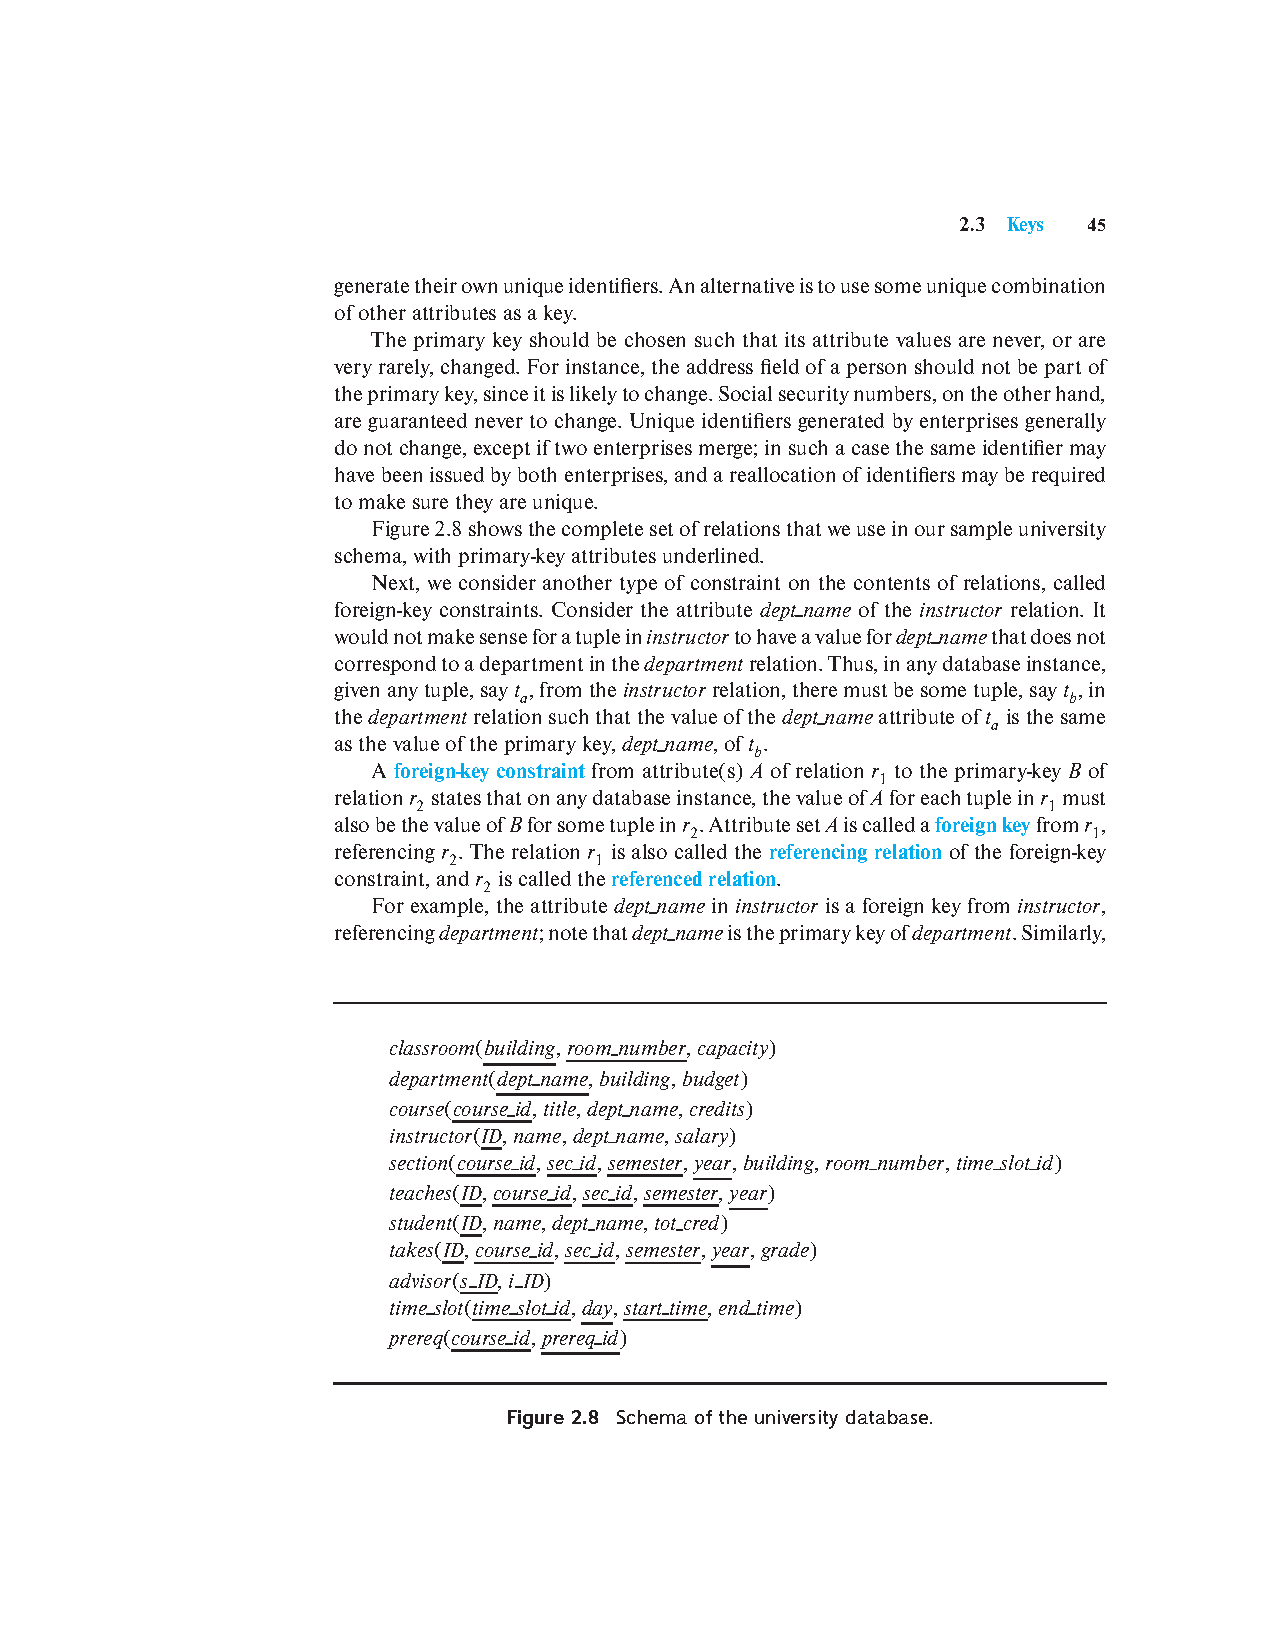
\includegraphics[width=\textwidth, trim={5.50cm 4.50cm 2.90cm 16.50cm}, clip]{figures/db_schema_prime}
\end{frame}

\begin{frame}{Schema Diagram for University Database}
    \centering
    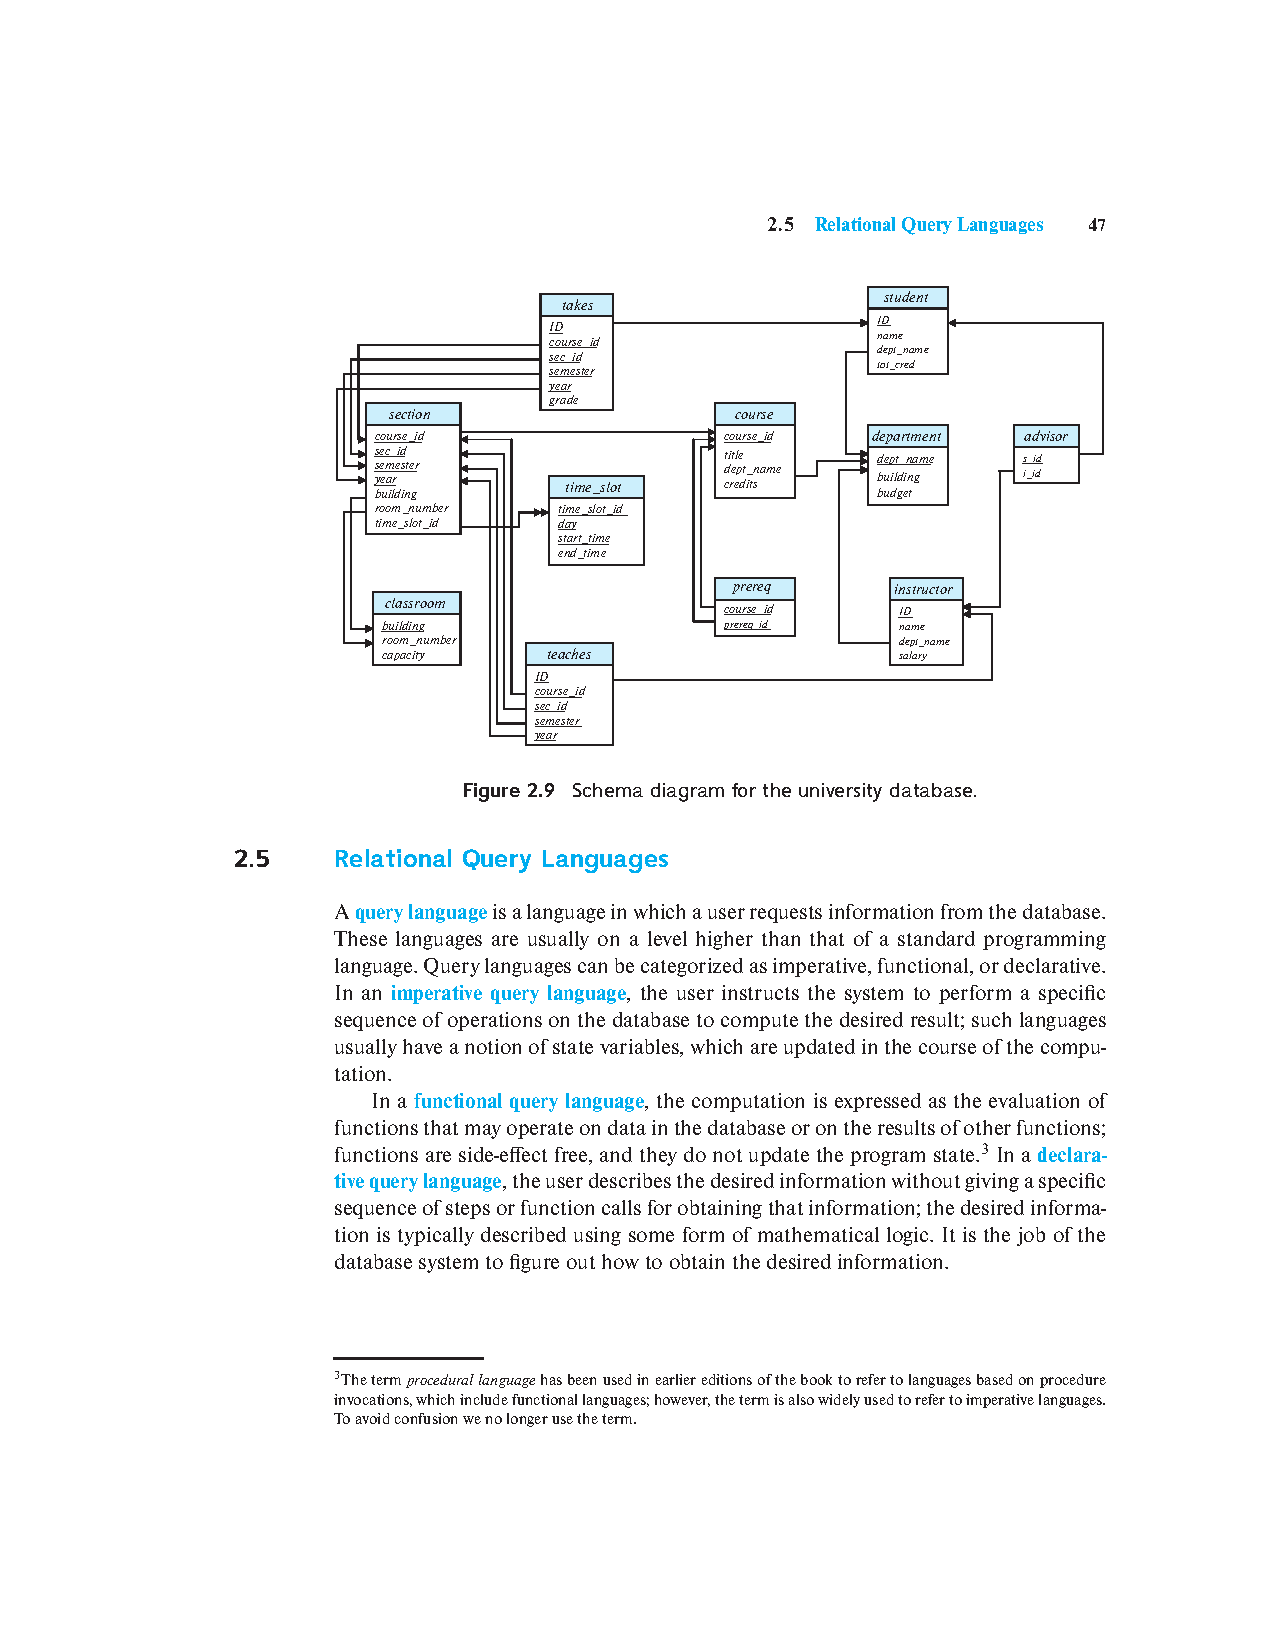
\includegraphics[width=\textwidth, trim={5.50cm 15.30cm 2.90cm 4.85cm}, clip]{figures/db_schema}
\end{frame}

\begin{frame}{Relational Query Languages}
    \begin{itemize}
        \item Procedural vs Non-procedural, or declarative.
        \item ``Pure'' languages:
        \begin{itemize}
            \item Relational algebra.
            \item Tuple relational calculus.
            \item Domain relational calculus.
        \end{itemize}
        \item The above 3 pure languages are equivalent in computing power.
        \item We will concentrate in this chapter on relational algebra:
        \begin{itemize}
            \item Not turning-machine equivalent.
            \item Consist of 6 basic operations.
        \end{itemize}
    \end{itemize}
\end{frame}

\begin{frame}{Relational Algebra}
    \begin{itemize}
        \item A procedural language consisting of a set of operations that take one or two relations as input and produce a new relation as their result.
        \item Six basic operators:
        \begin{itemize}
            \item select: $\sigma$
            \item project: $\Pi$
            \item union: $\cup$
            \item difference: $-$
            \item cartesian product: $\times$
            \item rename: $\rho$
        \end{itemize}
    \end{itemize}
\end{frame}

\begin{frame}{Select Operation}
    \begin{itemize}
        \item The \textbf{\texttt{select}} operation selects tuples that satisfy a given predicate.
        \item Notation: { \LARGE $\sigma_p (r)$ }.
        \item $p$ is called the \textbf{selection predicate}.
        \item Example: 
        \begin{itemize}
            \item Statement: ``Select those tuples of the instructor relation where the instructor is in the `Physics' department.''
            \item Query: 
                {\large
                $$
                    \sigma_{dept\_name = \text{`Physics'}} (instructor)
                $$}
            \item Result:\\
                \vspace{2mm}
                \centering
                \begin{tabular}{| l | l | l | l |}
                \hline
                 ID & name & dept\_name & salary \\
                 \hline
                 22222 & Einstein & Physics & 95000 \\
                 \hline
                 33456 & Gold & Physics & 87000 \\
                 \hline
                \end{tabular}
        \end{itemize}
    \end{itemize}
\end{frame}

\begin{frame}{Select Operation (Cont.)}
    \begin{itemize}
        \item We allow comparisons using $=$, $\neq$, $>$, $\geq$, $<$, $\leq$ in the selection predicate.
        \item We can combine several predicates into a larger predicate by using connectives: $\wedge$ \textbf{and}, $\vee$ \textbf{or}, $\neg$ \textbf{not}. 
        \item Example: ``Find the instructors in Physics with a salary greater than \$90000.''
        \item Solution: $$
            \sigma_{\text{dept\_name }=\text{ `Physics' } \wedge \text{ salary } > \text{ 90000}}(instructor)
        $$
        \item Then select predicate may include comparisons between two attributes.
        \begin{itemize}
            \item Example: ``Find all departments whose name is the same as their building name.''
            \item Solution: $$
                \sigma_{\text{dept\_name } = \text{ building}}(department)
            $$
        \end{itemize}
    \end{itemize}
\end{frame}

\begin{frame}{Project Operation}
    \begin{itemize}
        \item A unary operation that returns its argument relation, with certain attributes left out.
        \item Notation: { \LARGE $\Pi_{A_1, A_2, A_3, \ldots, A_k} (r)$ } where $A_1, A_2, \ldots, A_k$ are attribute names and $r$ is a relation name.
        \item The result is defined as the relation of $k$ columns obtained by erasing the columns that are not listed.
        \item Duplicate rows removed from result, since relations are sets.
    \end{itemize}
\end{frame}

\begin{frame}{Project Operation (Cont.)}
    \begin{itemize}
        \item Example: ``Eliminate the dept\_name attribute of instructor.''
        \item Query: $$
            \Pi_{\text{ID, name, salary}}(instructor)
        $$
        \item Result: 
    \end{itemize}
    \centering
    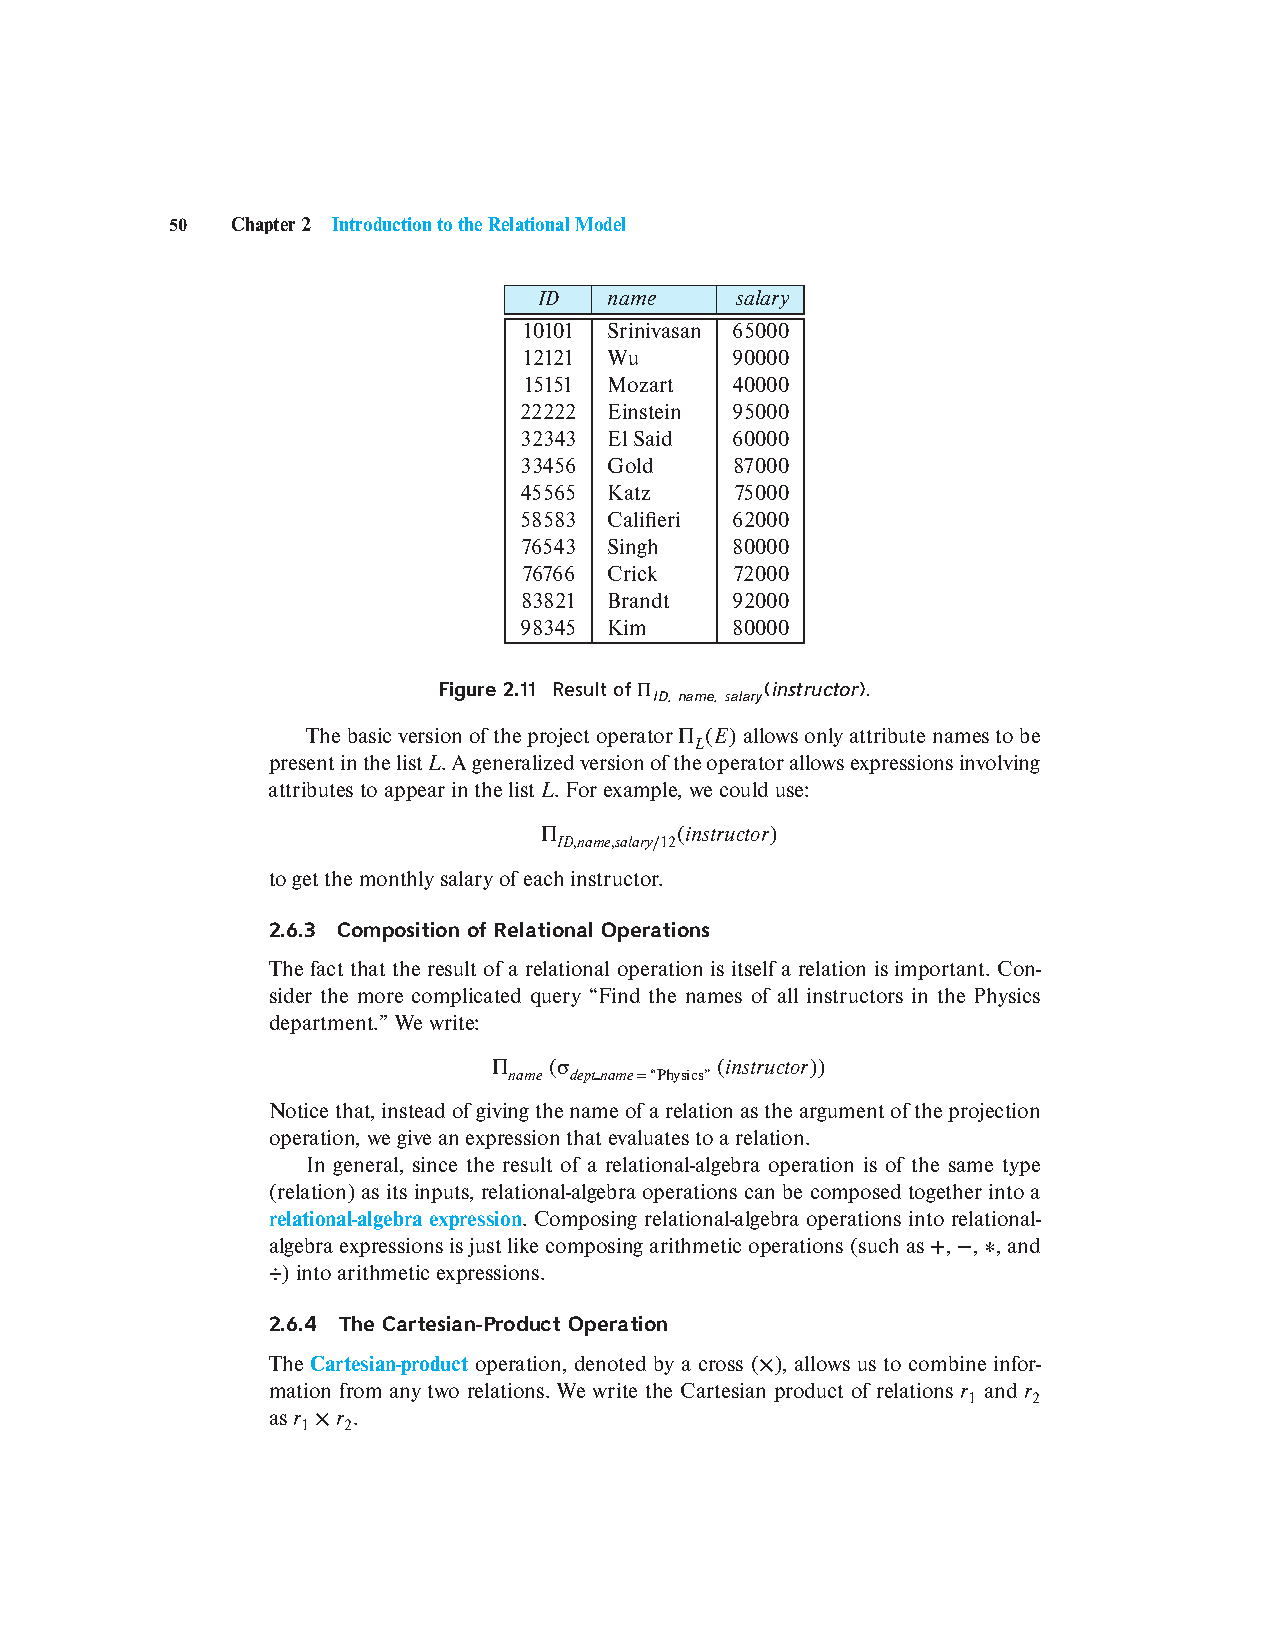
\includegraphics[width=0.75\textwidth, trim={5.50cm 17.00cm 5.00cm 4.75cm}, clip]{figures/db_project}
\end{frame}

\begin{frame}{Composition of Relational Operations}
    \begin{itemize}
        \item The result of a relational-algebra operation is a relation itself and therefore relational-algebra operations can be composed together into a \textbf{relational-algebra expression}.
        \item Consider the query: ``Find the names of all instructors in the Physics department.''
        {\Large
        $$
            \Pi_{\text{name}}(\sigma_{\text{dept\_name } = \text{ `Physics'}} (instructor))
        $$}
        \item Instead of giving the name of a relation as the argument of the projection operation, we give an expression that evaluates to a relation.
    \end{itemize}
\end{frame}

\begin{frame}{Cartesian-Product Operation}
    \begin{itemize}
        \item The Cartesian-Product operation (denoted by $\times$) allows us to combine information from any two relations.
        \item Example: the cartesian product of the relations \textit{instructor} and \textit{teaches} is written as:
        {\Large
            $$
                instructor \times teaches
            $$
        }
        \item We construct a tuple of the result out of each possible pair of tuples: one from the \textit{instructor} relation and one from the \textit{teaches} relation (see next slide).
        \item Since the instructor \textit{ID} appears in both relations, we distinguish between these attribute by attaching to the attribute the name of the relation from which the attribute originally came.
        \begin{itemize}
            \item \textit{instructor.ID}
            \item \textit{teaches.ID}
        \end{itemize}
    \end{itemize}
\end{frame}

\begin{frame}{The instructor $\times$ teaches table}
    \centering
    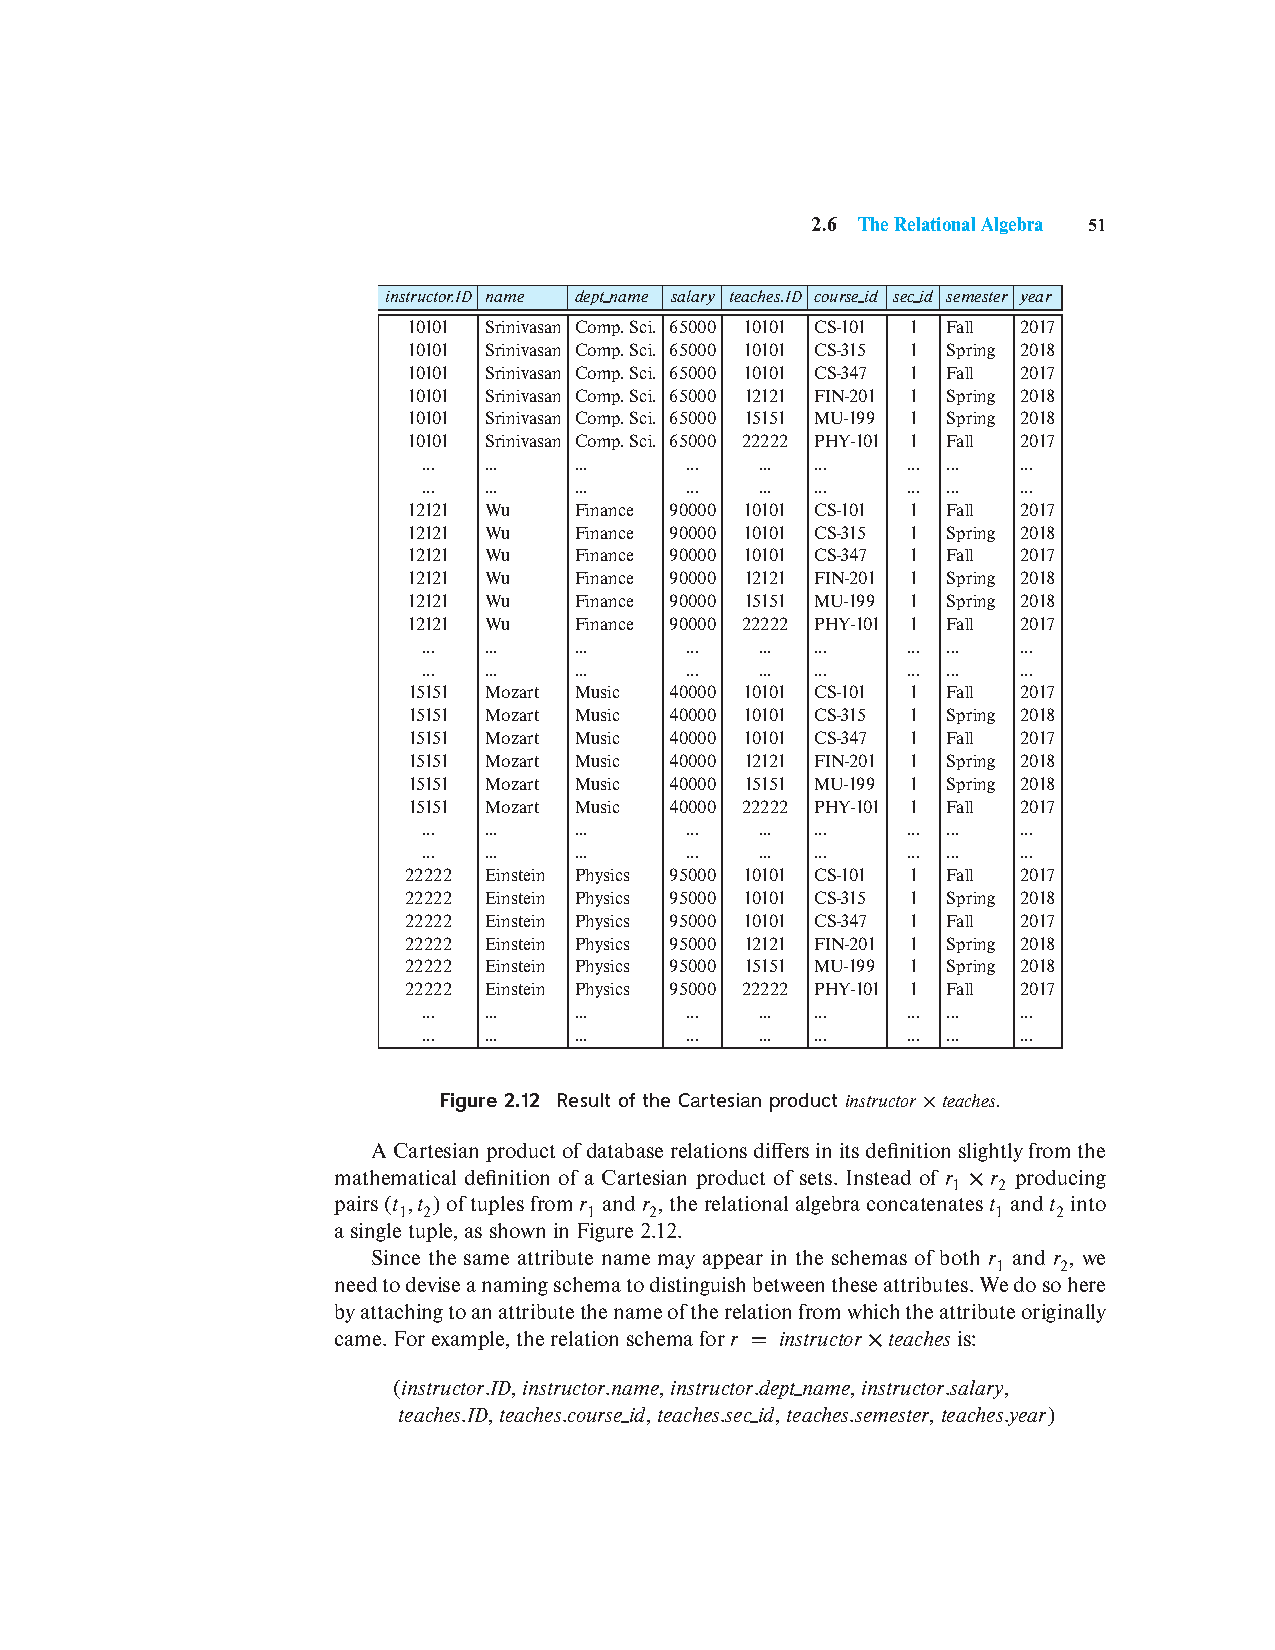
\includegraphics[width=0.70\textwidth, trim={6.40cm 10.15cm 3.60cm 4.80cm}, clip]{figures/db_cartesian}
\end{frame}

\begin{frame}{Join Operation}
    \begin{itemize}
        \item The Cartesian-Product
        $$
            instructor \times teaches
        $$
        associates every tuple of \textit{instructor} with every tuple of \textit{teaches}.
        \begin{itemize}
            \item Most of the resulting rows have information about instructors who did NOT teach a particular course.
        \end{itemize}
        \item To get only those tuples of ``$instructor \times teaches$'' that pertain to instructors and the courses that they taught, we write:
        {\Large
            $$
                \sigma_{\text{instructor.ID } = \text{ teaches.ID}}( instructor \times teaches )
            $$
        }
        \item The result of this expression is shown in the next slide.
    \end{itemize}
\end{frame}

\begin{frame}{Join Operation (Cont.)}
    \centering
    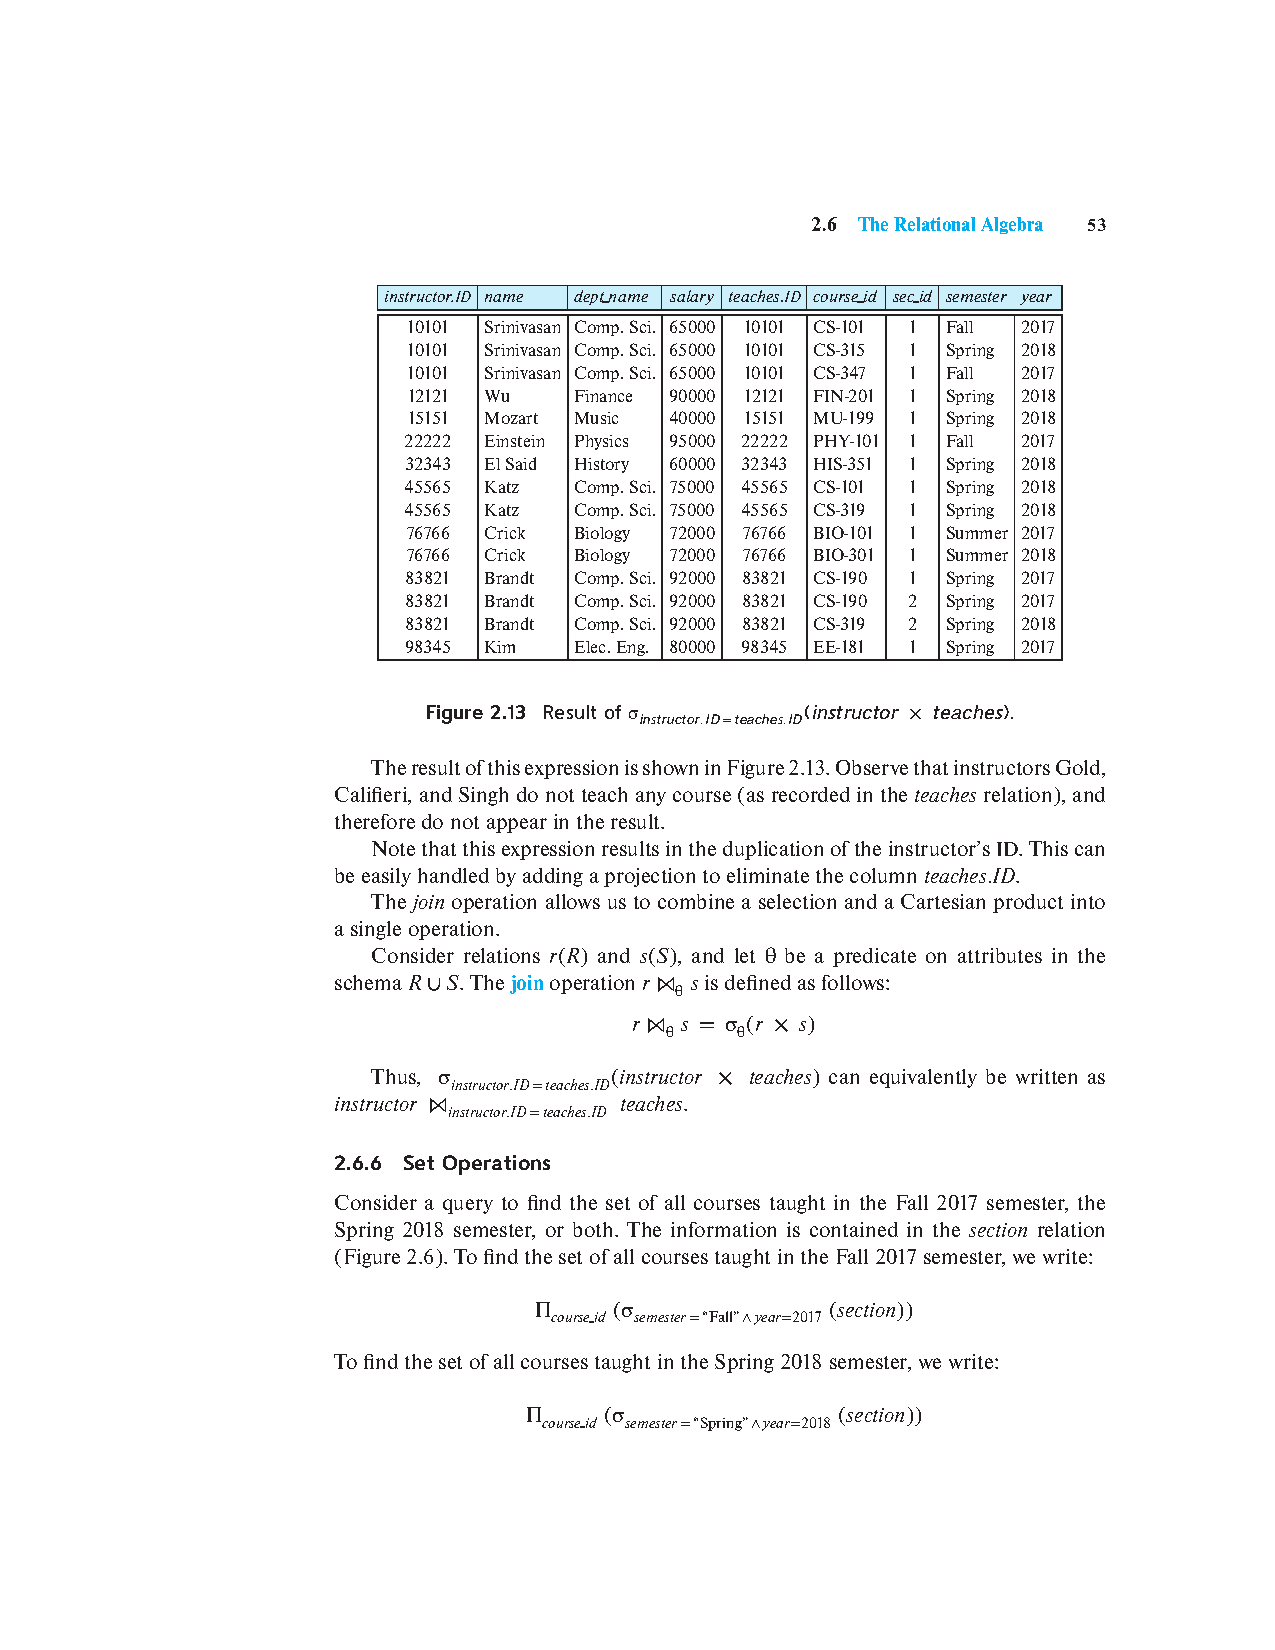
\includegraphics[width=\textwidth, trim={6.35cm 16.75cm 3.55cm 4.80cm}, clip]{figures/db_join}
\end{frame}

\begin{frame}{Join Operation (Cont.)}
    \begin{itemize}
        \item The Join operation allows us to combine a select operation and a cartesian-product operation into a single operation.
        \item Consider relations $r(R)$ and $s(S)$.
        \item Let ``theta'' be a predicate on attributes in the schema $R$ ``union'' $S$.  The join operation $r \Join_\theta s$ is defined as follows:
        {\Large
            $$
                r \Join_\theta s = \sigma_\theta (r \times s)
            $$
        }
        \item Thus
        {\Large
            $$
                \sigma_{\text{instructor.ID } = \text{ teaches.ID}}( instructor \times teaches )
            $$
        }
        \item Can equivalent be written as:
        {\Large
            $$
                instructor \Join_{\text{instructor.ID } = \text{ teaches.ID}} teaches 
            $$
        }
    \end{itemize}
\end{frame}

\begin{frame}{Union Operation}
    \begin{itemize}
        \item The union operation allows us to combine two relations.
        \item Notation: {\Large $r \cup s$}.
        \item For $r \cup s$ to be valid:
        \begin{enumerate}
            \item $r$,$s$ must have the same \textbf{arity} (same number of attributes).
            \item The attributes domain must be \textbf{compatible} (i.e. $2^{nd}$ column of $r$ deals with the same type of values as does the $2^{nd}$ column of $s$).
        \end{enumerate}
        \item Example: ``Find all courses taught in the Fall 2017 semester, or in the Spring 2018 semester, or in both''.
        \item Query:
        \begin{equation*}
            \begin{split}
                \Pi_{\text{course\_id}} (\sigma_{ \text{semester } = \text{ `Fall' } \wedge \text{ year } = \text{ 2017 } } (section) ) & \text{ } \cup \\
                \Pi_{\text{course\_id}} (\sigma_{ \text{semester } = \text{ `Spring' } \wedge \text{ year } = \text{ 2018 } } (section) ) & \\
            \end{split}
        \end{equation*}
    \end{itemize}
\end{frame}

\begin{frame}{Union Operation (Cont.)}
    \begin{itemize}
        \item Result of:
        \begin{equation*}
            \begin{split}
                \Pi_{\text{course\_id}} (\sigma_{ \text{semester } = \text{ `Fall' } \wedge \text{ year } = \text{ 2017 } } (section) ) & \text{ } \cup \\
                \Pi_{\text{course\_id}} (\sigma_{ \text{semester } = \text{ `Spring' } \wedge \text{ year } = \text{ 2018 } } (section) ) & \\
            \end{split}
        \end{equation*}
    \end{itemize}
    \centering
    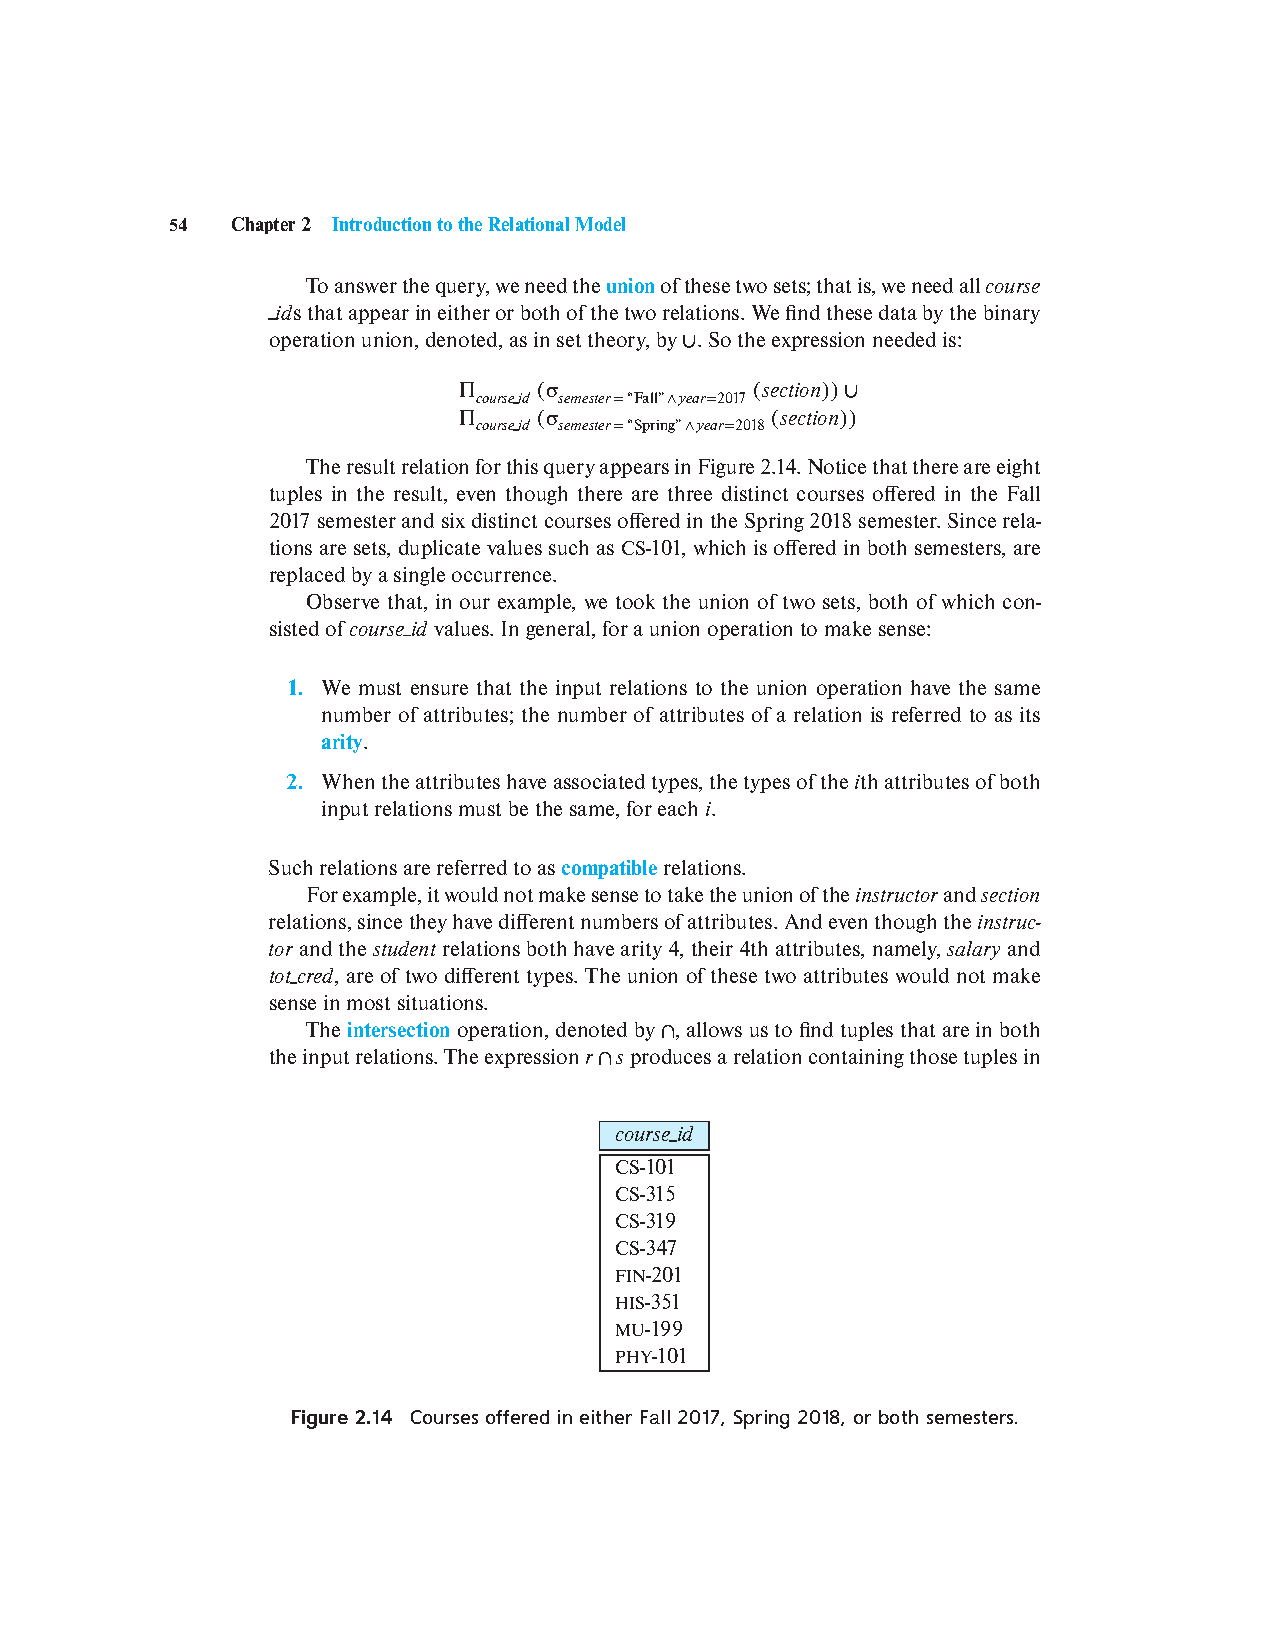
\includegraphics[width=0.75\textwidth, trim={6.35cm 4.50cm 6.00cm 18.95cm}, clip]{figures/db_union}
\end{frame}

\begin{frame}{Intersection Operation}
    \begin{itemize}
        \item The intersection operation allows us to find tuples that are in both the input relations.
        \item Notation: {\Large $r \cap s$}.
        \item For $r \cap s$ to be valid:
        \begin{enumerate}
            \item $r$,$s$ must have the same \textit{arity}.
            \item The attributes domain must be \textit{compatible}.
        \end{enumerate}
        \item Example: ``Find the set of all courses taught in the Fall 2017 and the Spring 2018 semesters''.
        \item Query:
        \begin{equation*}
            \begin{split}
                \Pi_{\text{course\_id}} (\sigma_{ \text{semester } = \text{ `Fall' } \wedge \text{ year } = \text{ 2017 } } (section) ) & \text{ } \cap \\
                \Pi_{\text{course\_id}} (\sigma_{ \text{semester } = \text{ `Spring' } \wedge \text{ year } = \text{ 2018 } } (section) ) & \\
            \end{split}
        \end{equation*}
    \end{itemize}
    \centering
    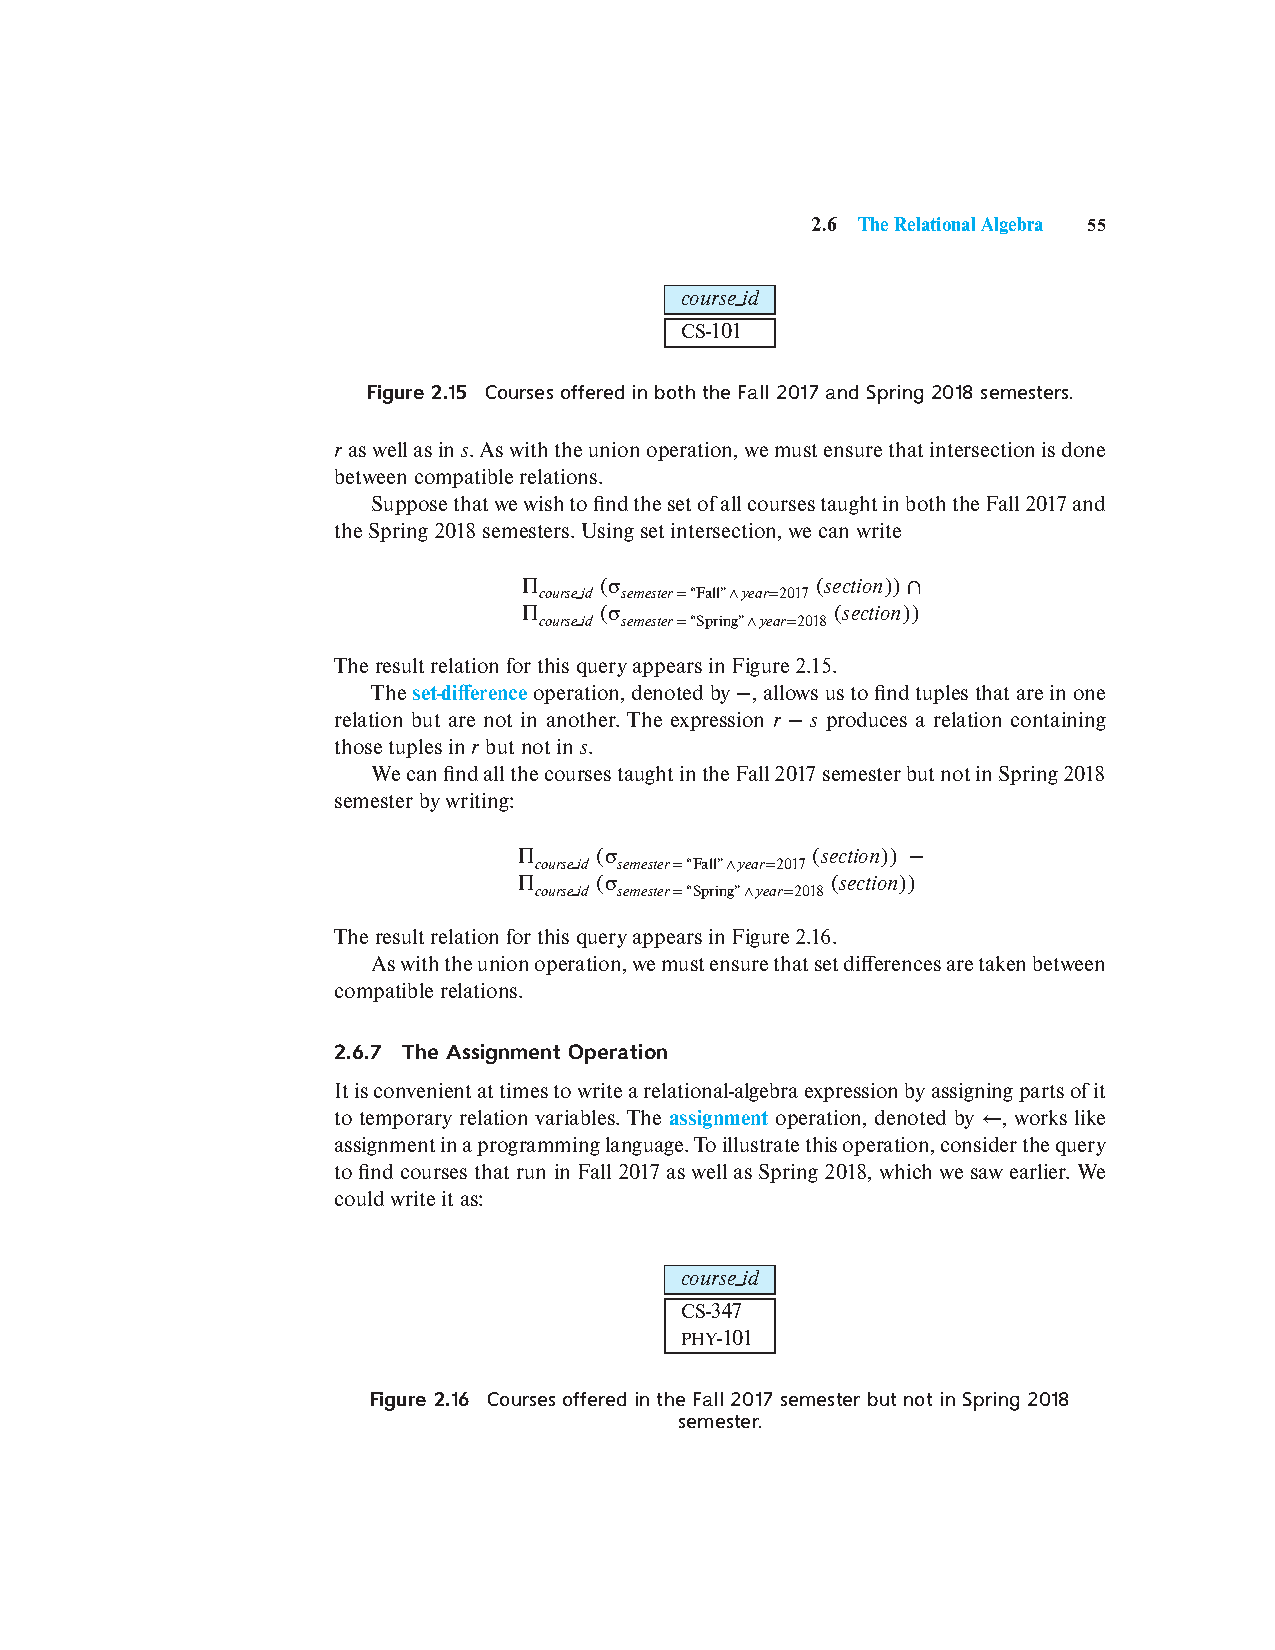
\includegraphics[width=0.40\textwidth, trim={9.50cm 21.50cm 8.00cm 4.50cm}, clip]{figures/db_intersection}    
\end{frame}

\begin{frame}{Difference Operation}
    \begin{itemize}
        \item The difference operation allows us to find tuples that are in one relation but are not in another.
        \item Notation: {\Large $r - s$}.
        \item For $r - s$ to be valid:
        \begin{enumerate}
            \item $r$,$s$ must have the same \textit{arity}.
            \item The attributes domain must be \textit{compatible}.
        \end{enumerate}
        \item Example: ``Find the set of all courses taught in the Fall 2017 semester, but not in the Spring 2018 semester''.
        \item Query:
        \begin{equation*}
            \begin{split}
                \Pi_{\text{course\_id}} (\sigma_{ \text{semester } = \text{ `Fall' } \wedge \text{ year } = \text{ 2017 } } (section) ) & \text{ } - \\
                \Pi_{\text{course\_id}} (\sigma_{ \text{semester } = \text{ `Spring' } \wedge \text{ year } = \text{ 2018 } } (section) ) & \\
            \end{split}
        \end{equation*}
    \end{itemize}
    \centering
    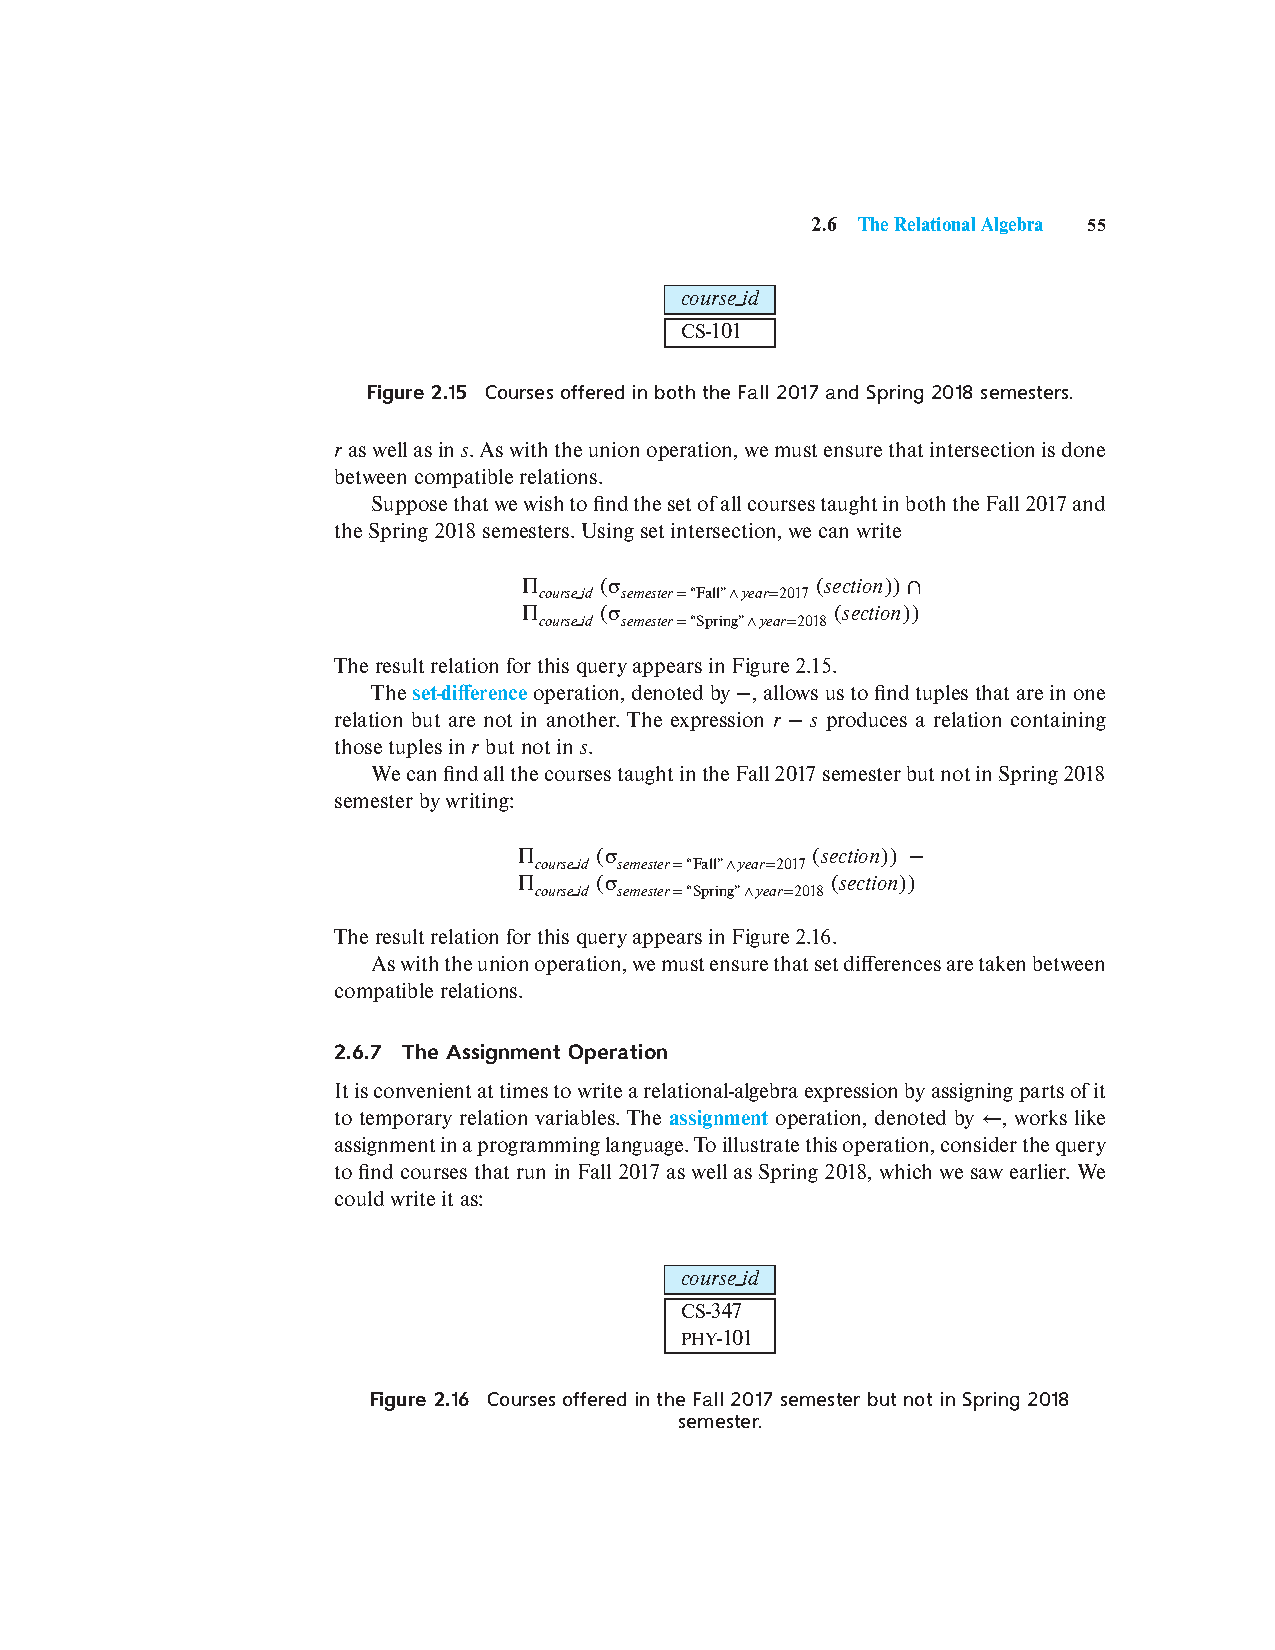
\includegraphics[width=0.45\textwidth, trim={9.50cm 4.50cm 7.50cm 21.00cm}, clip]{figures/db_intersection}    
\end{frame}

\begin{frame}{The Assignment Operation}
    \begin{itemize}
        \item It is convenient at times to write a relational-algebra expression by assigning part of it to temporary relation variable.
        \item The assignment operation is denoted by $\leftarrow$ and works like assignment in a programming language.
        \item Example: ``Find all instructors in the ``Physics'' and ``Music'' department.
        \begin{align*}
            physics &\leftarrow \sigma_{\text{dept\_name } = \text{ `Physics' }} (instructor) \\
            music &\leftarrow \sigma_{\text{dept\_name } = \text{ `Music' }} (instructor) \\
            physics &\cap music \\
        \end{align*}
        \item With the assignment operation, a query can be written as a sequential program consisting of a series of assignments followed by an expression whose value is displayed as the result of the query.
    \end{itemize}
\end{frame}

\begin{frame}{The Rename Operation}
    \begin{itemize}
        \item The results of relational-algebra expressions do not have a name that we can use to refer to them. The rename operator, $\rho$, is provided for that purpose.
        \item The expression:
            $$
                {\rho_x(E) }
            $$
            returns the result of expression $E$ under the name $x$.
        \item Another form of the rename operation:
            $$
                {\rho_{x(A_1, A_2, \ldots, A_n)}(E) }
            $$
    \end{itemize}
\end{frame}

\begin{frame}{Equivalent Queries}
    \begin{itemize}
        \item There are more than one way to write a query in relational algebra.
        \item Example: ``Find information about courses taught by instructors in the Physics department with salary greater than \$90,000.''
        \item Query 1: 
            $$
                \sigma_{\text{dept\_name } = \text{ `Physics' } \wedge \text{ salary } > \text{ 90000} } (instructor)
            $$
        \item Query 2: 
            $$
                \sigma_{\text{dept\_name } = \text{ `Physics' }} ( \sigma_{ \text{ salary } > \text{ 90000} } (instructor) )
            $$
        \item The two queries are not identical; they are, however, equivalent -- they give the same result on any database.
    \end{itemize}
\end{frame}

\begin{frame}{Equivalent Queries}
    \begin{itemize}
        \item There are more than one way to write a query in relational algebra.
        \item Example: ``Find information about courses taught by instructors in the Physics department.''
        \item Query 1: 
            $$
                \sigma_{\text{dept\_name } = \text{ `Physics' }} (instructor \Join_{\text{instructor.ID } = \text{ teaches.ID }} teaches )
            $$
        \item Query 2: 
            $$
                (\sigma_{\text{dept\_name } = \text{ `Physics' }} instructor) \Join_{\text{instructor.ID } = \text{ teaches.ID }} teaches 
            $$
        \item The two queries are not identical; they are, however, equivalent -- they give the same result on any database.
    \end{itemize}
\end{frame}



\begin{frame}{}
\end{frame}

\section*{Takeaways}

\begin{frame}{}
    \centering
    \Huge End of Chapter 2.
\end{frame}

\begin{frame}{Database System Concepts}
    \centering
    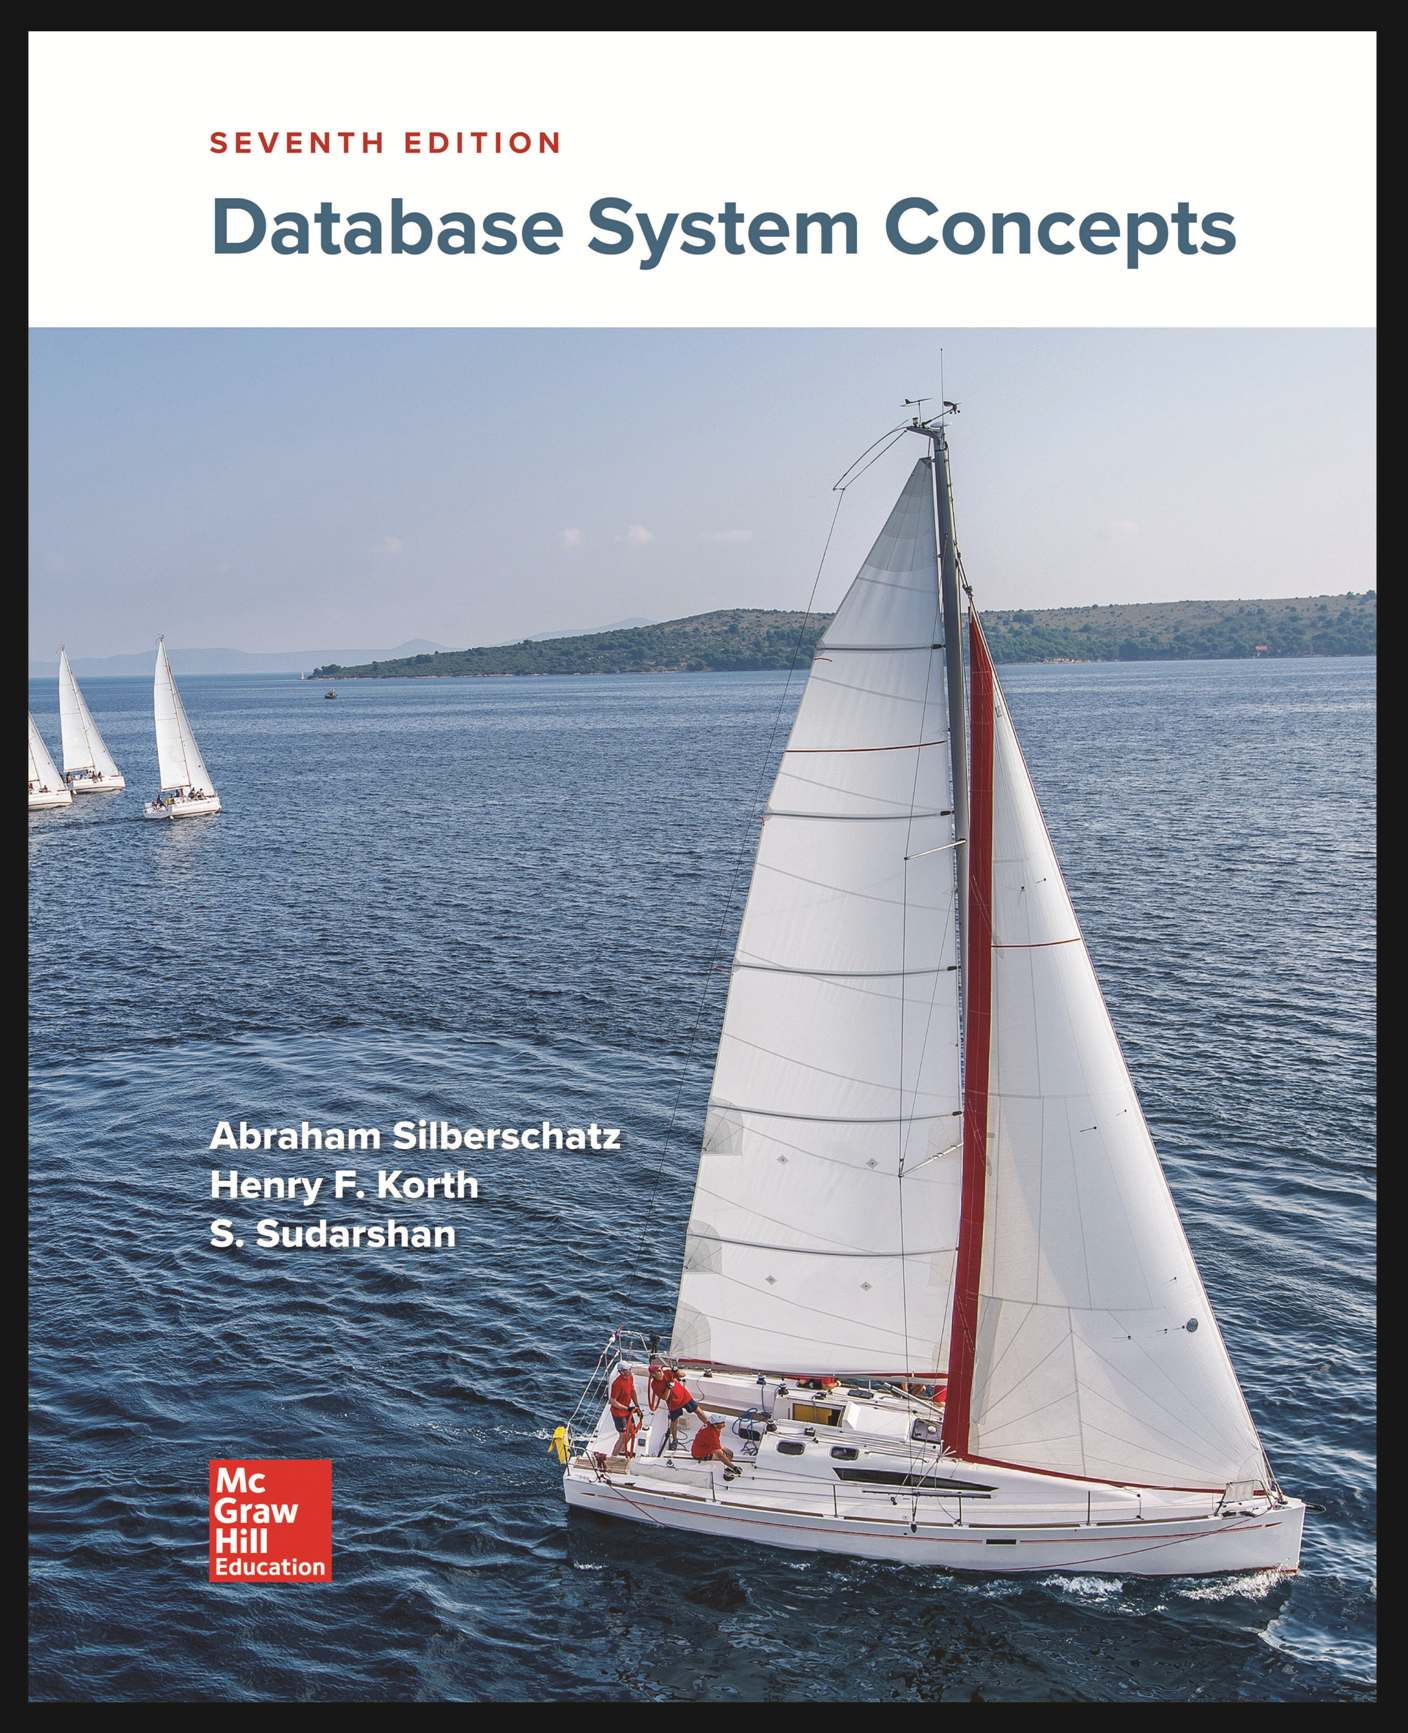
\includegraphics[width=0.5\textwidth]{figures/book_cover.jpg} \\
    \vspace{5mm}
    {
        \tiny
        Content has been extracted from \textit{Database System Concepts}, Seventh Edition, by Silberschatz, Korth and Sudarshan. Mc Graw Hill Education. 2019.\\
        Visit \url{https://db-book.com/}.\\
    }
\end{frame}

\end{document}
